%% Adaptado a partir de :
%%    abtex2-modelo-trabalho-academico.tex, v-1.9.2 laurocesar
%% para ser um modelo para os trabalhos no IFSP-SPO

\documentclass[
    % -- opções da classe memoir --
    12pt,               % tamanho da fonte
    openright,          % capítulos começam em pág ímpar (insere página vazia caso preciso)
    %twoside,            % para impressão em verso e anverso. Oposto a oneside
    oneside,
    a4paper,            % tamanho do papel. 
    % -- opções da classe abntex2 --
    %chapter=TITLE,     % títulos de capítulos convertidos em letras maiúsculas
    %section=TITLE,     % títulos de seções convertidos em letras maiúsculas
    %subsection=TITLE,  % títulos de subseções convertidos em letras maiúsculas
    %subsubsection=TITLE,% títulos de subsubseções convertidos em letras maiúsculas
    % Opções que não devem ser utilizadas na versão final do documento
    %draft,              % para compilar mais rápido, remover na versão final
    %MODELO,             % indica que é um documento modelo então precisa dos geradores de texto
    %TODO,                indica que deve apresentar lista de pendencias 
    % -- opções do pacote babel --
    english,            % idioma adicional para hifenização
    brazil              % o último idioma é o principal do documento
    ]{ifsp-spo-inf-ctds}

        
% ---

% --- 
% CONFIGURAÇÕES DE PACOTES
% --- 
%\usepackage{etoolbox}
%\patchcmd{\thebibliography}{\chapter*}{\section*}{}{}
\usepackage{float}
\usepackage{quoting} %para citações com várias linhas
% ---
% Informações de dados para CAPA e FOLHA DE ROSTO
% ---
\titulo{Website de Vagas de Estágio}

% Trabalho individual
%\autor{JOSÉ BRAZ DE ARAUJO}

% Trabalho em Equipe
% ver também https://github.com/abntex/abntex2/wiki/FAQ#como-adicionar-mais-de-um-autor-ao-meu-projeto
\renewcommand{\imprimirautor}{
\begin{tabular}{lr}
Bruna da Silva Pires & SP3056651 \\
Daniel Roberto Pereira & SP3046702 \\
Igor Nathan de Oliveira Rocha & SP305263X \\
Leonardo Marques da Silva & SP3052591 \\
Lucas Lima de Santana & SP3046559 \\
Marcelo Carlos Olimpio Junior &SP3046583 \\
\end{tabular}
}


\tipotrabalho{Projeto da Disciplina PI1A5}

\disciplina{PI1A5 - Projeto Integrado I}

\preambulo{Desenho de aplicação para desenvolvimento na disciplina de Projeto Integrado I no 1º semestre de 2022.}

\data{2022}

% Definir o que for necessário e comentar o que não for necessário
% Utilizar o Nome Completo, abntex tem orientador e coorientador
% então vão ser utilizados na definição de professor
\renewcommand{\orientadorname}{Professor:}
\orientador{Carlos Henrique Veríssimo Pereira}
%\renewcommand{\coorientadorname}{Professor:}
%\coorientador{NOME COMPLETO DO PROFESSOR2}



% ---



% ---
% Configurações de aparência do PDF final


% informações do PDF
\makeatletter
\hypersetup{
        %pagebackref=true,
        pdftitle={\@title}, 
        pdfauthor={\@author},
        pdfsubject={\imprimirpreambulo},
        pdfcreator={LaTeX with abnTeX2},
        pdfkeywords={abnt}{latex}{abntex}{abntex2}{trabalho acadêmico}, 
        colorlinks=true,            % false: boxed links; true: colored links
        linkcolor=blue,             % color of internal links
        citecolor=blue,             % color of links to bibliography
        filecolor=magenta,              % color of file links
        urlcolor=blue,
        bookmarksdepth=4
}
\makeatother
% --- 

% ---

% ----
% Início do documento
% ----
\begin{document}

% Retira espaço extra obsoleto entre as frases.
\frenchspacing 

\pretextual

% ---
% Capa - Para proposta a folha de rosto é suficiente pois é mais completa.
% ---
\imprimirfolhaderosto
\newpage


% ---
% inserir lista de ilustrações
% ---
\pdfbookmark[0]{\listfigurename}{lof}
\listoffigures*
\cleardoublepage
% ---

% ---
% inserir lista de quadros
% ---
\pdfbookmark[0]{\listofquadrosname}{loq}
\listofquadros*
\cleardoublepage
% ---

% ---
% inserir lista de abreviaturas e siglas
% ATENCAO o SHARELATEX/OVERLEAF GERA O GLOSSARIO SOMENTE UMA VEZ
% CASO SEJA FEITA ALGUMA ALTERAÇÃO NA LISTA DE SIGLAS É NECESSARIO UTILIZAR A OPÇÃO :
% "Clear Cached Files" DISPONIVEL NA VISUALIZAÇÃO DOS LOGS 
% ---
% https://www.sharelatex.com/learn/Glossaries

\ifdef{\printnoidxglossary}{
    \printnoidxglossary[type=\acronymtype,title=Lista de abreviaturas e siglas,style=siglas]
    \cleardoublepage
}{}

% ---
% inserir o sumario
% ---
\pdfbookmark[0]{\contentsname}{toc}
\tableofcontents*
\cleardoublepage
% ---
% ----------------------------------------------------------
% ELEMENTOS TEXTUAIS
% ----------------------------------------------------------
\textual

% ----------------------------------------------------------
% INTRODUÇÃO
% ----------------------------------------------------------
\chapter[Introdução]{Introdução}

Nesse capítulo serão mostrados os principais pontos do nosso projeto, os objetivos e quais os problemas que queremos solucionar com nossa aplicação.

% ----------------------------------------------------------
% JUSTIFICATIVA
% ----------------------------------------------------------
% ----------------------------------------------------------
% JUSTIFICATIVA
% ----------------------------------------------------------
\section{Justificativa}
%O problema encontrado
Existe, na contemporaneidade, uma grande dificuldade em adquirir experiência profissional através da prática de estágio, muitas vezes obrigatória no projeto pedagógico de curso das universidades. Tal problema se dá por meio das plataformas que disponibilizam tais vagas, porém com uma certa cobrança injusta em relação a habilidades que o candidato precisa possuir previamente. É também notável que existe uma certa dificuldade de conexão entre a empresa e o candidato, que muitas vezes não obtém o retorno sobre o processo de seleção da vaga.

% ----------------------------------------------------------
% PROPOSTA
% ----------------------------------------------------------
% ----------------------------------------------------------
% PROPOSTA
% ----------------------------------------------------------
\section{Proposta de solução}
%Descrição geral da nossa proposta
Tendo em vista os problemas anteriormente descritos, \emph{EstagiEI} é um sistema para aproximar novos estudantes e empresas com vagas de estágio disponíveis, de modo que os candidatos possam receber indicações de vagas condizentes com seu perfil e empresas recebam recomendações de candidatos possivelmente adequados às vagas anunciadas.


% ----------------------------------------------------------
% OBJETIVOS
% ----------------------------------------------------------
% ----------------------------------------------------------
% OBJETIVOS
% ----------------------------------------------------------
\section{Objetivos}
Com nossa solução buscamos promover um meio de conexão mais direto entre os estudantes em busca de estágio e empresas que buscam interessados em suas vagas de estágio alinhados com o perfil buscado. Através do sistema de recomendações, tantos os estudantes quanto as empresas têm papel ativo no processo de encontrar um(a) estudante/vaga ideal, cujas as competências e perfil sejam condizentes com o que é procurado.

Podemos definir nosso objetivo principal como:
\begin{itemize}
		\item Ser uma aplicação onde de fato os estudantes encontrem vagas que condizem com a realidade de um estagiário.
\end{itemize}

A partir do nosso objetivo principal, podemos explicitar alguns objetivos adjacentes:

\begin{itemize}
	\item Ser um \emph{website} de fácil usabilidade, onde os estudantes encontrem vagas sem passar por longos processos seletivos.
	\item Pensar sempre na experiência dos usuários, de modo que a aplicação seja simples e efetiva ao mesmo tempo.
\end{itemize}

% ----------------------------------------------------------
% CONCORRÊNCIA
% ----------------------------------------------------------
% ----------------------------------------------------------
% CONCORRÊNCIA
% ----------------------------------------------------------
\section{Análise de Concorrentes}
Para a elaboração da proposta, foram verificadas algumas soluções já existentes no mercado. A partir disso, as soluções que mais se assemelham com a proposta foram o \textit{Companhia de Estágios}, \textit{Cia de Talentos} e
\textit{Nube}. Com base neste levantamento, podemos observar algumas intersecções de funcionalidades oferecidas. O quadro \ref{concorrentes} permite a melhor visualização deste levantamento.

\begin{quadro}[h]
\caption{Comparação dos aplicativos concorrentes}
\centering
\ABNTEXfontereduzida
 % \resizebox{\columnwidth}{!}{%
    \begin{tabular}{| p{0.30\linewidth} | c | c | c | c |}
      \hline
      \thead[l]{Funcionalidades} & \thead{Cia de \\Estágios} & \thead{Cia de \\ Talentos} & \thead{Nube} & \thead{Nosso Proj.}\\
      \hline
      Login/Cadastro. & x & x & x & x\\
      \hline
      Aplicar em uma vaga. & x & x & x & x\\
      \hline
      Notificação a cada mudança do status no processo seletivo. &  &  & x & x\\
      \hline
      Recomendação de vagas e/ou empresas aos estudantes de acordo com as suas características. & & & & x\\
      \hline
      Recomendação de estudantes mais compatíveis com as vagas registradas pelas empresas, de acordo com as características da vaga e da empresa. & & & & x\\
      \hline
      Simplificação de contato via \emph{WhatsApp}. & & & & x\\
      \hline
      Denúncias de vagas incoerentes com a realidade. & & & & x\\
      \hline
      \emph{Feedback} de empresas pós-entrevista.  & & & & x\\
      \hline
      
    \end{tabular}
 % }
  \fonte{Os Autores}
  \label{concorrentes}
\end{quadro}




% ----------------------------------------------------------
% INTRODUÇÃO
% ----------------------------------------------------------
\chapter[Introdução]{Introdução}

Nesse capítulo serão mostrados os principais pontos do nosso projeto, os objetivos e quais os problemas que queremos solucionar com nossa aplicação.

% ----------------------------------------------------------
% JUSTIFICATIVA
% ----------------------------------------------------------
% ----------------------------------------------------------
% JUSTIFICATIVA
% ----------------------------------------------------------
\section{Justificativa}
%O problema encontrado
Existe, na contemporaneidade, uma grande dificuldade em adquirir experiência profissional através da prática de estágio, muitas vezes obrigatória no projeto pedagógico de curso das universidades. Tal problema se dá por meio das plataformas que disponibilizam tais vagas, porém com uma certa cobrança injusta em relação a habilidades que o candidato precisa possuir previamente. É também notável que existe uma certa dificuldade de conexão entre a empresa e o candidato, que muitas vezes não obtém o retorno sobre o processo de seleção da vaga.

% ----------------------------------------------------------
% PROPOSTA
% ----------------------------------------------------------
% ----------------------------------------------------------
% PROPOSTA
% ----------------------------------------------------------
\section{Proposta de solução}
%Descrição geral da nossa proposta
Tendo em vista os problemas anteriormente descritos, \emph{EstagiEI} é um sistema para aproximar novos estudantes e empresas com vagas de estágio disponíveis, de modo que os candidatos possam receber indicações de vagas condizentes com seu perfil e empresas recebam recomendações de candidatos possivelmente adequados às vagas anunciadas.


% ----------------------------------------------------------
% OBJETIVOS
% ----------------------------------------------------------
% ----------------------------------------------------------
% OBJETIVOS
% ----------------------------------------------------------
\section{Objetivos}
Com nossa solução buscamos promover um meio de conexão mais direto entre os estudantes em busca de estágio e empresas que buscam interessados em suas vagas de estágio alinhados com o perfil buscado. Através do sistema de recomendações, tantos os estudantes quanto as empresas têm papel ativo no processo de encontrar um(a) estudante/vaga ideal, cujas as competências e perfil sejam condizentes com o que é procurado.

Podemos definir nosso objetivo principal como:
\begin{itemize}
		\item Ser uma aplicação onde de fato os estudantes encontrem vagas que condizem com a realidade de um estagiário.
\end{itemize}

A partir do nosso objetivo principal, podemos explicitar alguns objetivos adjacentes:

\begin{itemize}
	\item Ser um \emph{website} de fácil usabilidade, onde os estudantes encontrem vagas sem passar por longos processos seletivos.
	\item Pensar sempre na experiência dos usuários, de modo que a aplicação seja simples e efetiva ao mesmo tempo.
\end{itemize}

% ----------------------------------------------------------
% CONCORRÊNCIA
% ----------------------------------------------------------
% ----------------------------------------------------------
% CONCORRÊNCIA
% ----------------------------------------------------------
\section{Análise de Concorrentes}
Para a elaboração da proposta, foram verificadas algumas soluções já existentes no mercado. A partir disso, as soluções que mais se assemelham com a proposta foram o \textit{Companhia de Estágios}, \textit{Cia de Talentos} e
\textit{Nube}. Com base neste levantamento, podemos observar algumas intersecções de funcionalidades oferecidas. O quadro \ref{concorrentes} permite a melhor visualização deste levantamento.

\begin{quadro}[h]
\caption{Comparação dos aplicativos concorrentes}
\centering
\ABNTEXfontereduzida
 % \resizebox{\columnwidth}{!}{%
    \begin{tabular}{| p{0.30\linewidth} | c | c | c | c |}
      \hline
      \thead[l]{Funcionalidades} & \thead{Cia de \\Estágios} & \thead{Cia de \\ Talentos} & \thead{Nube} & \thead{Nosso Proj.}\\
      \hline
      Login/Cadastro. & x & x & x & x\\
      \hline
      Aplicar em uma vaga. & x & x & x & x\\
      \hline
      Notificação a cada mudança do status no processo seletivo. &  &  & x & x\\
      \hline
      Recomendação de vagas e/ou empresas aos estudantes de acordo com as suas características. & & & & x\\
      \hline
      Recomendação de estudantes mais compatíveis com as vagas registradas pelas empresas, de acordo com as características da vaga e da empresa. & & & & x\\
      \hline
      Simplificação de contato via \emph{WhatsApp}. & & & & x\\
      \hline
      Denúncias de vagas incoerentes com a realidade. & & & & x\\
      \hline
      \emph{Feedback} de empresas pós-entrevista.  & & & & x\\
      \hline
      
    \end{tabular}
 % }
  \fonte{Os Autores}
  \label{concorrentes}
\end{quadro}



% ----------------------------------------------------------
% INTRODUÇÃO
% ----------------------------------------------------------
\chapter[Introdução]{Introdução}

Nesse capítulo serão mostrados os principais pontos do nosso projeto, os objetivos e quais os problemas que queremos solucionar com nossa aplicação.

% ----------------------------------------------------------
% JUSTIFICATIVA
% ----------------------------------------------------------
% ----------------------------------------------------------
% JUSTIFICATIVA
% ----------------------------------------------------------
\section{Justificativa}
%O problema encontrado
Existe, na contemporaneidade, uma grande dificuldade em adquirir experiência profissional através da prática de estágio, muitas vezes obrigatória no projeto pedagógico de curso das universidades. Tal problema se dá por meio das plataformas que disponibilizam tais vagas, porém com uma certa cobrança injusta em relação a habilidades que o candidato precisa possuir previamente. É também notável que existe uma certa dificuldade de conexão entre a empresa e o candidato, que muitas vezes não obtém o retorno sobre o processo de seleção da vaga.

% ----------------------------------------------------------
% PROPOSTA
% ----------------------------------------------------------
% ----------------------------------------------------------
% PROPOSTA
% ----------------------------------------------------------
\section{Proposta de solução}
%Descrição geral da nossa proposta
Tendo em vista os problemas anteriormente descritos, \emph{EstagiEI} é um sistema para aproximar novos estudantes e empresas com vagas de estágio disponíveis, de modo que os candidatos possam receber indicações de vagas condizentes com seu perfil e empresas recebam recomendações de candidatos possivelmente adequados às vagas anunciadas.


% ----------------------------------------------------------
% OBJETIVOS
% ----------------------------------------------------------
% ----------------------------------------------------------
% OBJETIVOS
% ----------------------------------------------------------
\section{Objetivos}
Com nossa solução buscamos promover um meio de conexão mais direto entre os estudantes em busca de estágio e empresas que buscam interessados em suas vagas de estágio alinhados com o perfil buscado. Através do sistema de recomendações, tantos os estudantes quanto as empresas têm papel ativo no processo de encontrar um(a) estudante/vaga ideal, cujas as competências e perfil sejam condizentes com o que é procurado.

Podemos definir nosso objetivo principal como:
\begin{itemize}
		\item Ser uma aplicação onde de fato os estudantes encontrem vagas que condizem com a realidade de um estagiário.
\end{itemize}

A partir do nosso objetivo principal, podemos explicitar alguns objetivos adjacentes:

\begin{itemize}
	\item Ser um \emph{website} de fácil usabilidade, onde os estudantes encontrem vagas sem passar por longos processos seletivos.
	\item Pensar sempre na experiência dos usuários, de modo que a aplicação seja simples e efetiva ao mesmo tempo.
\end{itemize}

% ----------------------------------------------------------
% CONCORRÊNCIA
% ----------------------------------------------------------
% ----------------------------------------------------------
% CONCORRÊNCIA
% ----------------------------------------------------------
\section{Análise de Concorrentes}
Para a elaboração da proposta, foram verificadas algumas soluções já existentes no mercado. A partir disso, as soluções que mais se assemelham com a proposta foram o \textit{Companhia de Estágios}, \textit{Cia de Talentos} e
\textit{Nube}. Com base neste levantamento, podemos observar algumas intersecções de funcionalidades oferecidas. O quadro \ref{concorrentes} permite a melhor visualização deste levantamento.

\begin{quadro}[h]
\caption{Comparação dos aplicativos concorrentes}
\centering
\ABNTEXfontereduzida
 % \resizebox{\columnwidth}{!}{%
    \begin{tabular}{| p{0.30\linewidth} | c | c | c | c |}
      \hline
      \thead[l]{Funcionalidades} & \thead{Cia de \\Estágios} & \thead{Cia de \\ Talentos} & \thead{Nube} & \thead{Nosso Proj.}\\
      \hline
      Login/Cadastro. & x & x & x & x\\
      \hline
      Aplicar em uma vaga. & x & x & x & x\\
      \hline
      Notificação a cada mudança do status no processo seletivo. &  &  & x & x\\
      \hline
      Recomendação de vagas e/ou empresas aos estudantes de acordo com as suas características. & & & & x\\
      \hline
      Recomendação de estudantes mais compatíveis com as vagas registradas pelas empresas, de acordo com as características da vaga e da empresa. & & & & x\\
      \hline
      Simplificação de contato via \emph{WhatsApp}. & & & & x\\
      \hline
      Denúncias de vagas incoerentes com a realidade. & & & & x\\
      \hline
      \emph{Feedback} de empresas pós-entrevista.  & & & & x\\
      \hline
      
    \end{tabular}
 % }
  \fonte{Os Autores}
  \label{concorrentes}
\end{quadro}



% ----------------------------------------------------------
% INTRODUÇÃO
% ----------------------------------------------------------
\chapter[Introdução]{Introdução}

Nesse capítulo serão mostrados os principais pontos do nosso projeto, os objetivos e quais os problemas que queremos solucionar com nossa aplicação.

% ----------------------------------------------------------
% JUSTIFICATIVA
% ----------------------------------------------------------
% ----------------------------------------------------------
% JUSTIFICATIVA
% ----------------------------------------------------------
\section{Justificativa}
%O problema encontrado
Existe, na contemporaneidade, uma grande dificuldade em adquirir experiência profissional através da prática de estágio, muitas vezes obrigatória no projeto pedagógico de curso das universidades. Tal problema se dá por meio das plataformas que disponibilizam tais vagas, porém com uma certa cobrança injusta em relação a habilidades que o candidato precisa possuir previamente. É também notável que existe uma certa dificuldade de conexão entre a empresa e o candidato, que muitas vezes não obtém o retorno sobre o processo de seleção da vaga.

% ----------------------------------------------------------
% PROPOSTA
% ----------------------------------------------------------
% ----------------------------------------------------------
% PROPOSTA
% ----------------------------------------------------------
\section{Proposta de solução}
%Descrição geral da nossa proposta
Tendo em vista os problemas anteriormente descritos, \emph{EstagiEI} é um sistema para aproximar novos estudantes e empresas com vagas de estágio disponíveis, de modo que os candidatos possam receber indicações de vagas condizentes com seu perfil e empresas recebam recomendações de candidatos possivelmente adequados às vagas anunciadas.


% ----------------------------------------------------------
% OBJETIVOS
% ----------------------------------------------------------
% ----------------------------------------------------------
% OBJETIVOS
% ----------------------------------------------------------
\section{Objetivos}
Com nossa solução buscamos promover um meio de conexão mais direto entre os estudantes em busca de estágio e empresas que buscam interessados em suas vagas de estágio alinhados com o perfil buscado. Através do sistema de recomendações, tantos os estudantes quanto as empresas têm papel ativo no processo de encontrar um(a) estudante/vaga ideal, cujas as competências e perfil sejam condizentes com o que é procurado.

Podemos definir nosso objetivo principal como:
\begin{itemize}
		\item Ser uma aplicação onde de fato os estudantes encontrem vagas que condizem com a realidade de um estagiário.
\end{itemize}

A partir do nosso objetivo principal, podemos explicitar alguns objetivos adjacentes:

\begin{itemize}
	\item Ser um \emph{website} de fácil usabilidade, onde os estudantes encontrem vagas sem passar por longos processos seletivos.
	\item Pensar sempre na experiência dos usuários, de modo que a aplicação seja simples e efetiva ao mesmo tempo.
\end{itemize}

% ----------------------------------------------------------
% CONCORRÊNCIA
% ----------------------------------------------------------
% ----------------------------------------------------------
% CONCORRÊNCIA
% ----------------------------------------------------------
\section{Análise de Concorrentes}
Para a elaboração da proposta, foram verificadas algumas soluções já existentes no mercado. A partir disso, as soluções que mais se assemelham com a proposta foram o \textit{Companhia de Estágios}, \textit{Cia de Talentos} e
\textit{Nube}. Com base neste levantamento, podemos observar algumas intersecções de funcionalidades oferecidas. O quadro \ref{concorrentes} permite a melhor visualização deste levantamento.

\begin{quadro}[h]
\caption{Comparação dos aplicativos concorrentes}
\centering
\ABNTEXfontereduzida
 % \resizebox{\columnwidth}{!}{%
    \begin{tabular}{| p{0.30\linewidth} | c | c | c | c |}
      \hline
      \thead[l]{Funcionalidades} & \thead{Cia de \\Estágios} & \thead{Cia de \\ Talentos} & \thead{Nube} & \thead{Nosso Proj.}\\
      \hline
      Login/Cadastro. & x & x & x & x\\
      \hline
      Aplicar em uma vaga. & x & x & x & x\\
      \hline
      Notificação a cada mudança do status no processo seletivo. &  &  & x & x\\
      \hline
      Recomendação de vagas e/ou empresas aos estudantes de acordo com as suas características. & & & & x\\
      \hline
      Recomendação de estudantes mais compatíveis com as vagas registradas pelas empresas, de acordo com as características da vaga e da empresa. & & & & x\\
      \hline
      Simplificação de contato via \emph{WhatsApp}. & & & & x\\
      \hline
      Denúncias de vagas incoerentes com a realidade. & & & & x\\
      \hline
      \emph{Feedback} de empresas pós-entrevista.  & & & & x\\
      \hline
      
    \end{tabular}
 % }
  \fonte{Os Autores}
  \label{concorrentes}
\end{quadro}



%\chapter{Processos modelados}
% Precisamos colocar isso agora msm?
\section{Recomendação de vagas para o estudante}
\subsection{Descrição}

\subsection{Diagrama BPMN}


\section{Recomendação de estudantes para vagas cadastradas}
\subsection{Descrição}

\subsection{Diagrama BPMN}


\section{Recomendação de empresas para o estudante}
\subsection{Descrição}

\subsection{Diagrama BPMN}


%% ---
% Conclusão (outro exemplo de capítulo sem numeração e presente no sumário)
% Dependendo do trabalho desenvolvido ele pode ter uma Conclusão ou Considerações finais
% Para trabalhos de disciplina utilizar Considerações Finais
% ---
\chapter{Considerações Finais}
% Exemplo de como adicionar linha adicional no sumário
%\addcontentsline{toc}{chapter}{Considerações Finais}
% Para definir sem número utilizar o asterisco
% Mas se tiver sub seção vai continuar a contagem do capítulo anterior
%\chapter{Considerações finais}



% ---
Além desse documento ser um modelo de como pode ser criado um documento em \LaTeX \space ele também apresenta diversas informações úteis para as disciplinas de projetos de informática do \ac{ifsp} e alguns elementos uteis para as monografias do curso de Pós Graduação em Gestão de \acs{ti} do \ac{ifsp}.

\explicacao{Um trabalho de disciplina não tem \enquote{Conclusão}}

\preencheComTexto


\explicacao{Exemplo de possíveis seções para monografia da pós graduação...}
\section{Resposta à Questão de Pesquisa}
\preencheComTexto

\section{Objetivos Propostos}
\preencheComTexto

\section{Contribuições Acadêmicas e Gerenciais}
\preencheComTexto

\section{Limitações da Pesquisa e Contribuições para Estudo}
\preencheComTexto



%Teste de citação para gerar referências no modelo.. \citeauthor{SCRUMGUIDE:2013}

% ----------------------------------------------------------
% Referências bibliográficas
% ----------------------------------------------------------
\bibliography{referencias}

% ----------------------------------------------------------
% Glossário
% ----------------------------------------------------------
%
%
\ifdef{\printnoidxglossary}{
    \addcontentsline{toc}{chapter}{GLOSSÁRIO}
    \printnoidxglossary[style=glossario]
    %\printglossaries
}{}

%% ----------------------------------------------------------
% Apêndices
% Documentos gerados pelo próprio autor
% ----------------------------------------------------------

% ---
% Inicia os apêndices
% ---
\begin{apendicesenv}

% Imprime uma página indicando o início dos apêndices
\partapendices

% ----------------------------------------------------------
\chapter{Publicações do BLog}
% ----------------------------------------------------------



% ----------------------------------------------------------
\chapter{Desenho da Aplicação}
% ----------------------------------------------------------


\end{apendicesenv}
% ---


%% ----------------------------------------------------------
% Anexos
% Documentos gerados por outros autores
% ----------------------------------------------------------

% ---
% Inicia os anexos
% ---
\begin{anexosenv}
\anexos
% Imprime uma página indicando o início dos anexos
\partanexos


% ----------------------------------------------------------
%\chapter{Nota dos headers}
% ----------------------------------------------------------
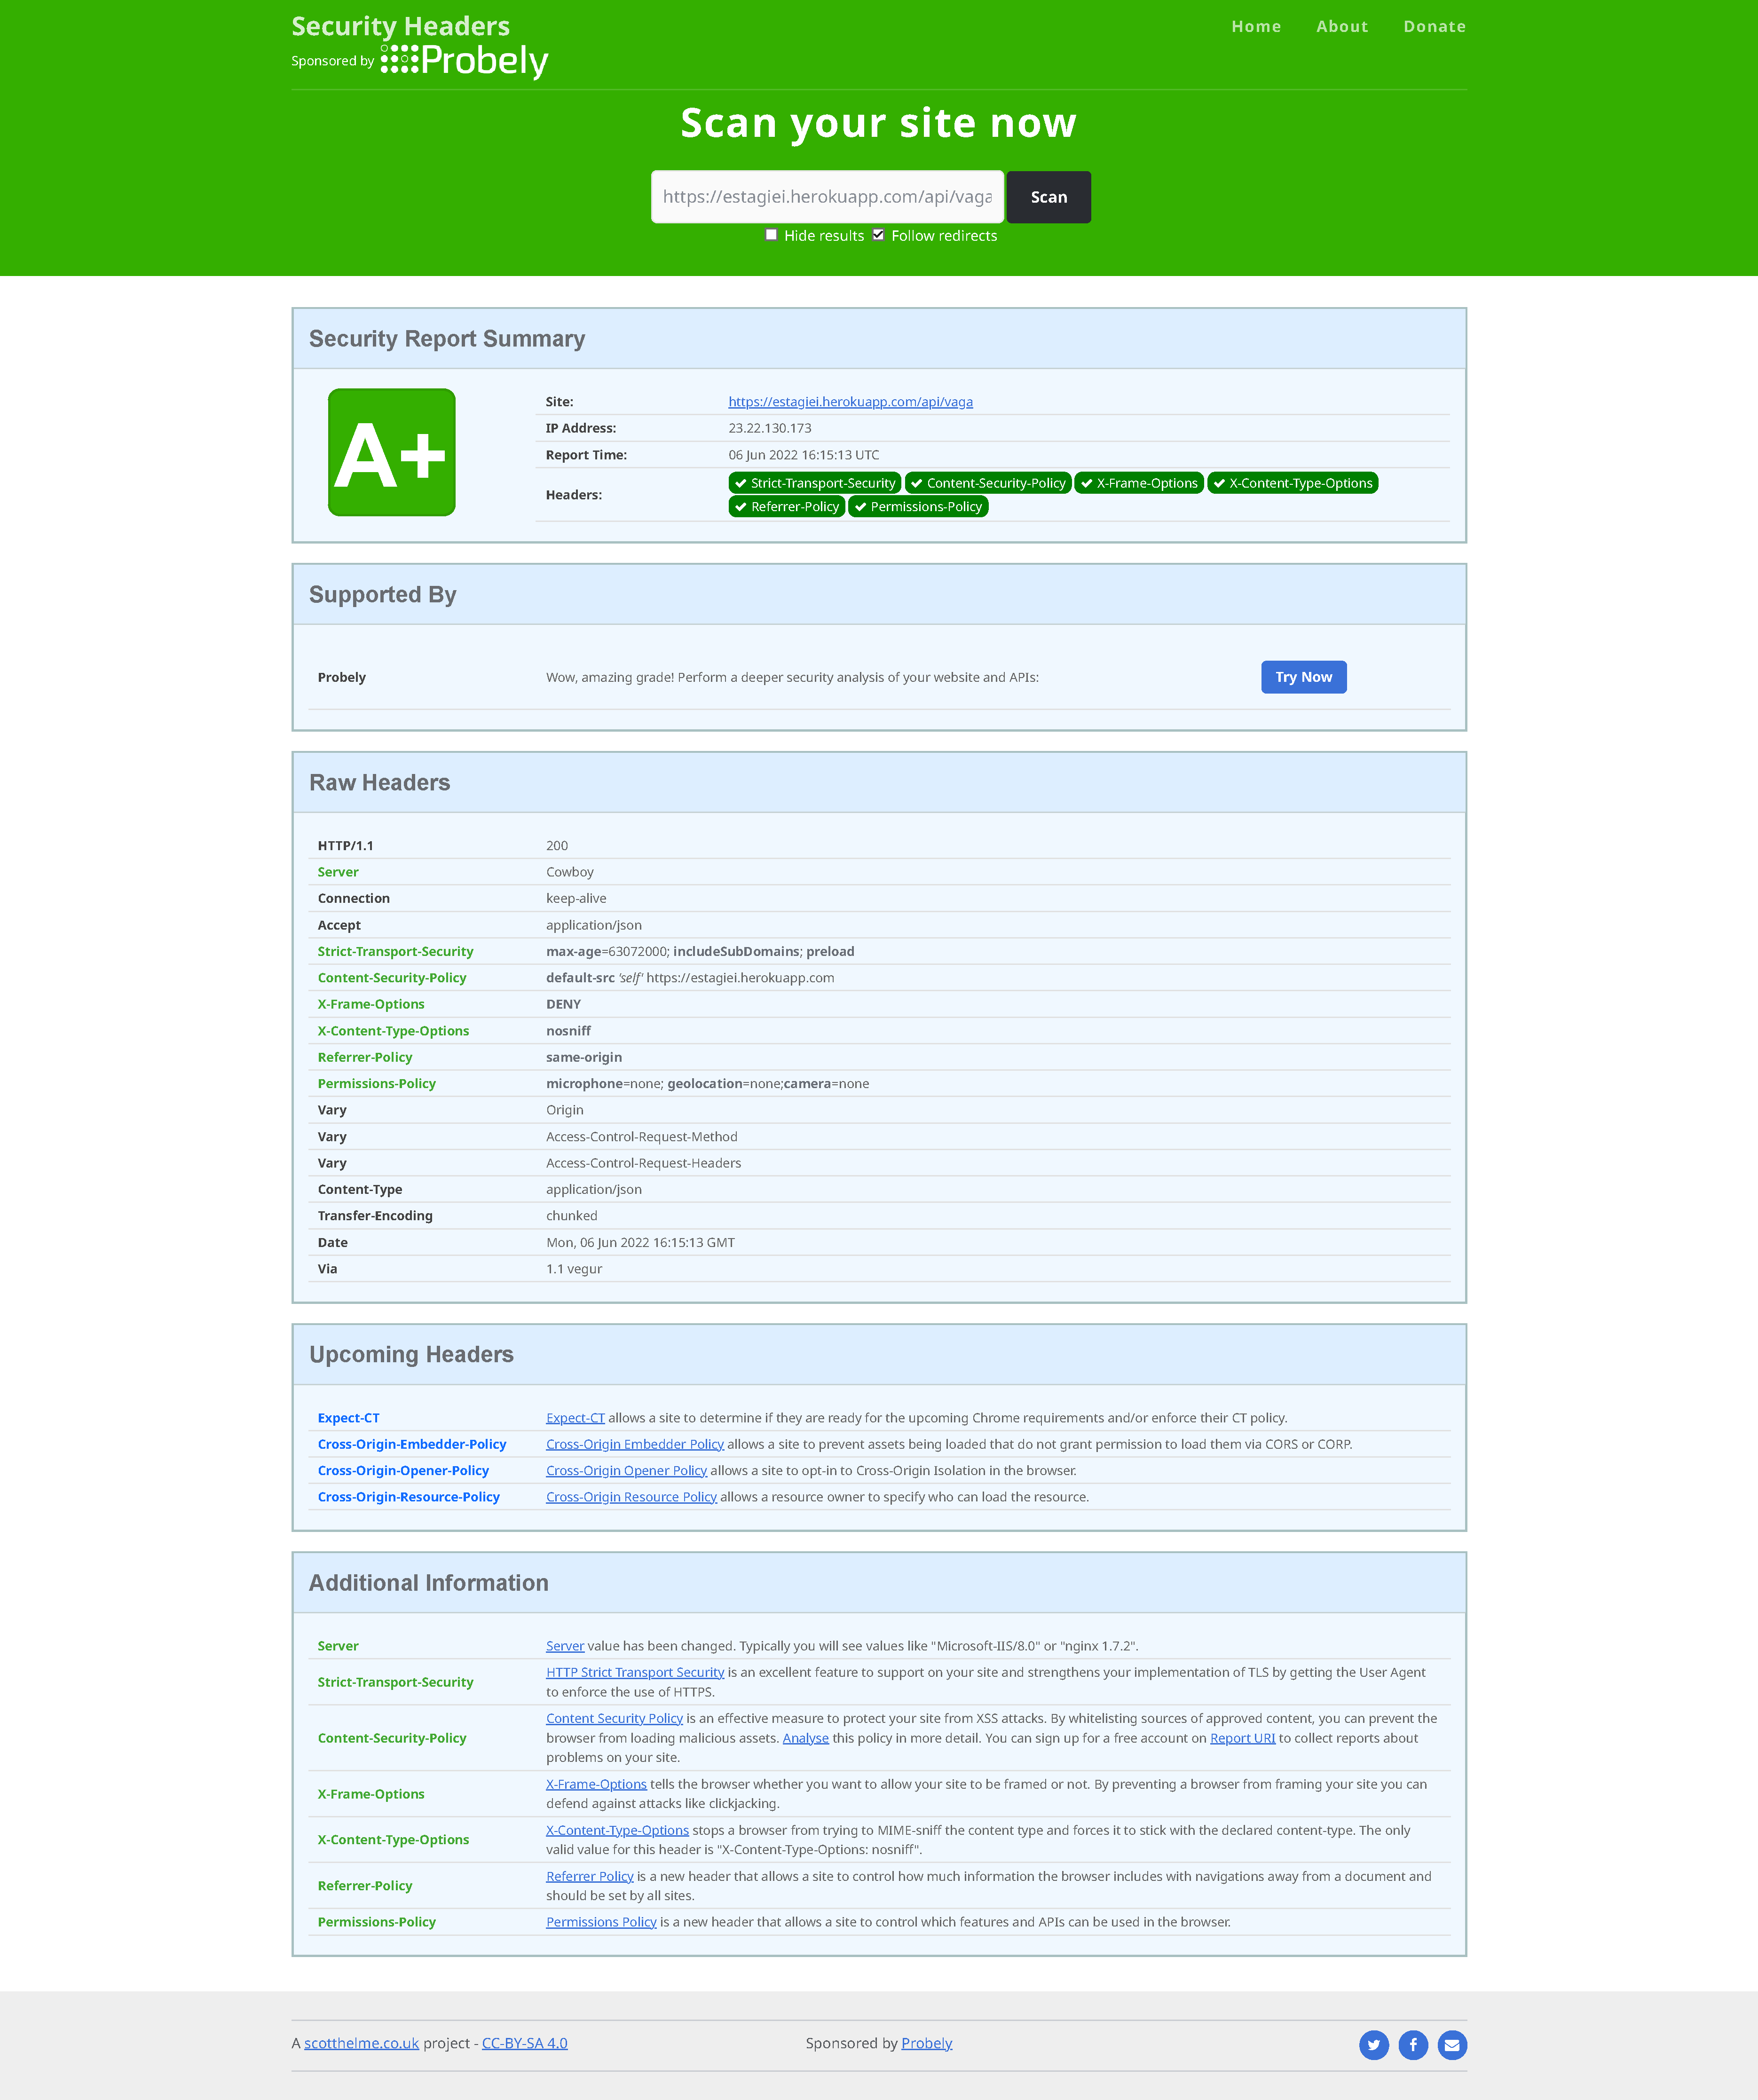
\includepdf[pages=1, scale=0.87, frame=true, pagecommand=\chapter{Nota dos headers}\label{scan-headers}]{../artefatos/scan-results-for-https-estagiei-herokuapp-com-api-vaga.pdf}

\begin{comment}
% ---
\chapter{Manual todonotes(parcial)}
\label{manual-todonotes}
% ---
\index{pdf}
% se pages = "-"  fica com arquivo completo
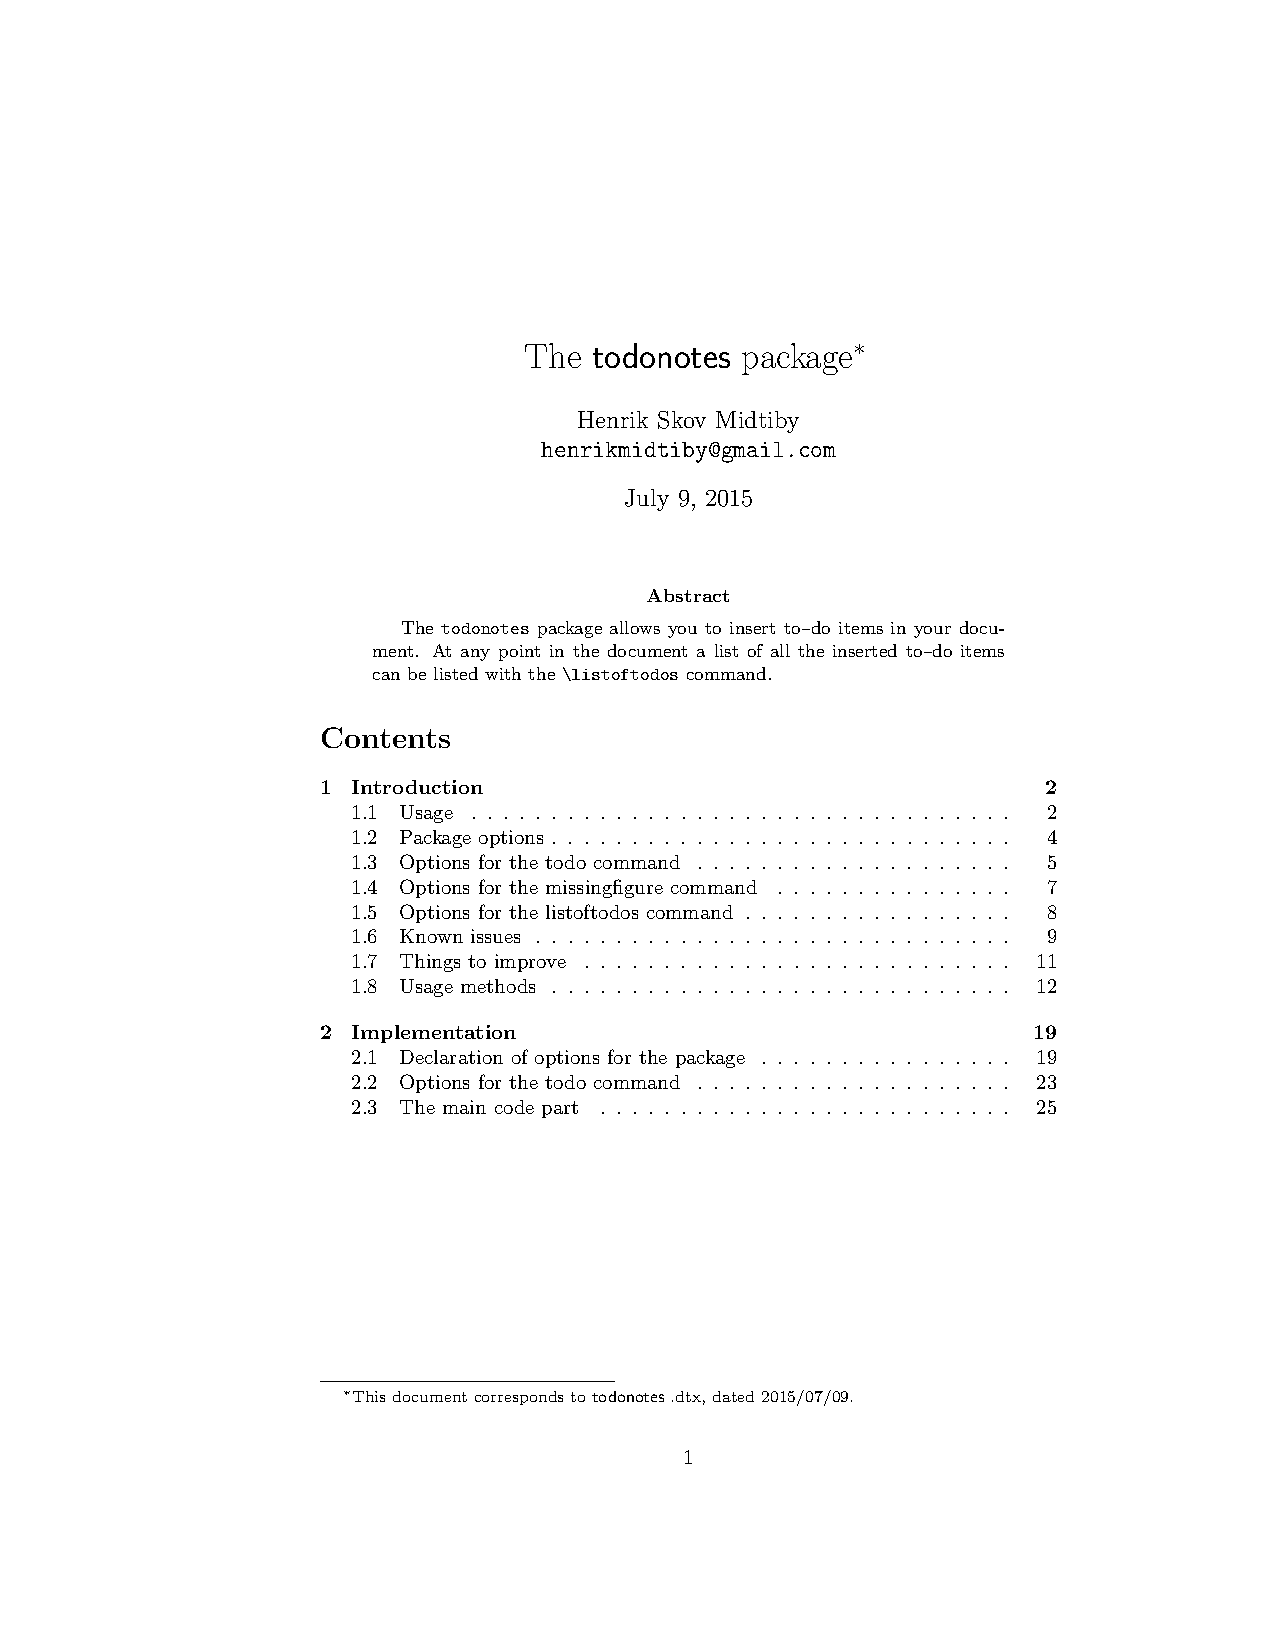
\includepdf[pages=1-3,scale=0.8,frame=true,pagecommand={}]{anexos/todonotes.pdf}

% ---
% Para incluir sem gerar a quebra de página inicial no anexo
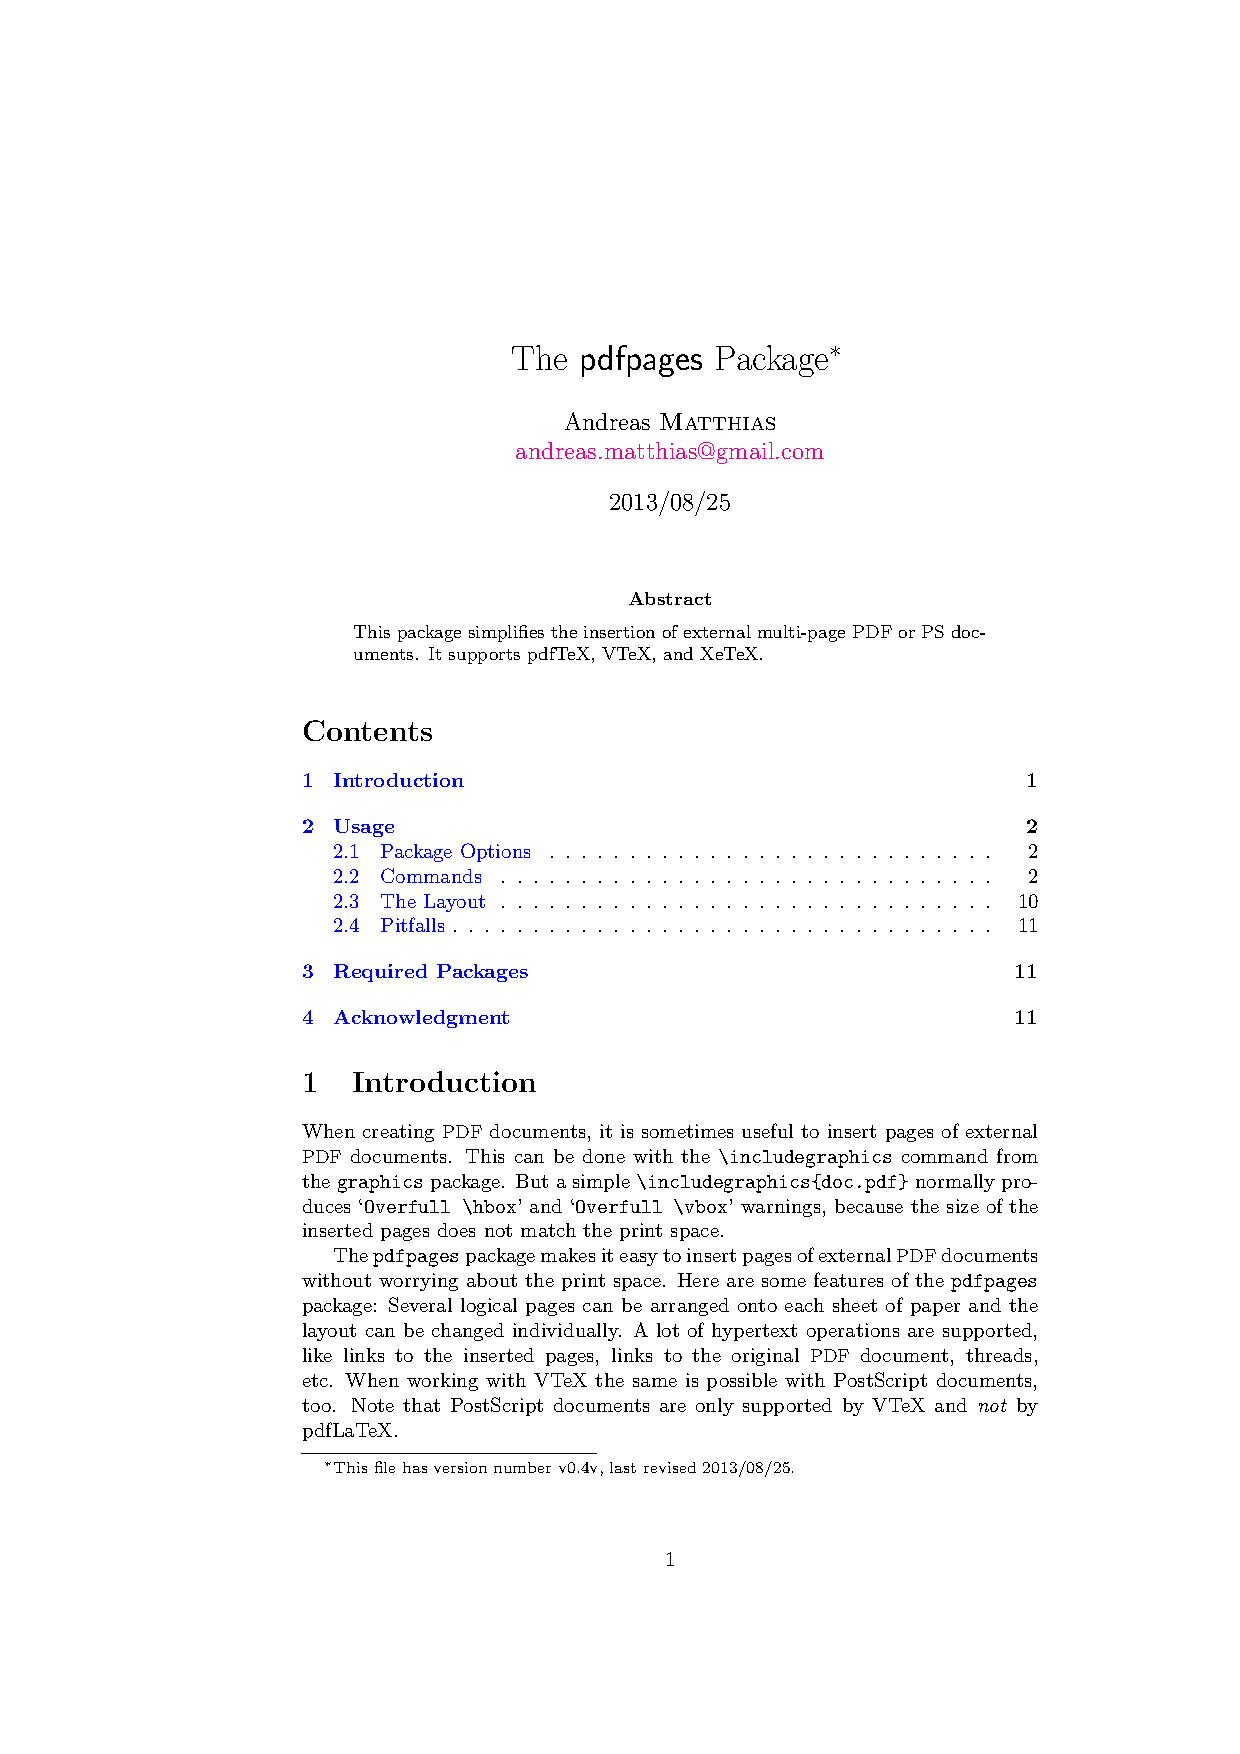
\includepdf[pages=1,scale=0.7,frame=true,pagecommand=\chapter{Manual pdfpages(parcial)}\label{manual-pdfpages}]{anexos/pdfpages.pdf}
\includepdf[pages=2-3,scale=0.8,frame=true,pagecommand={}]{anexos/pdfpages.pdf}

% ---
\chapter{Manual acronym(parcial)}
\index{pdf}
% somente algumas páginas para exemplo sem borda
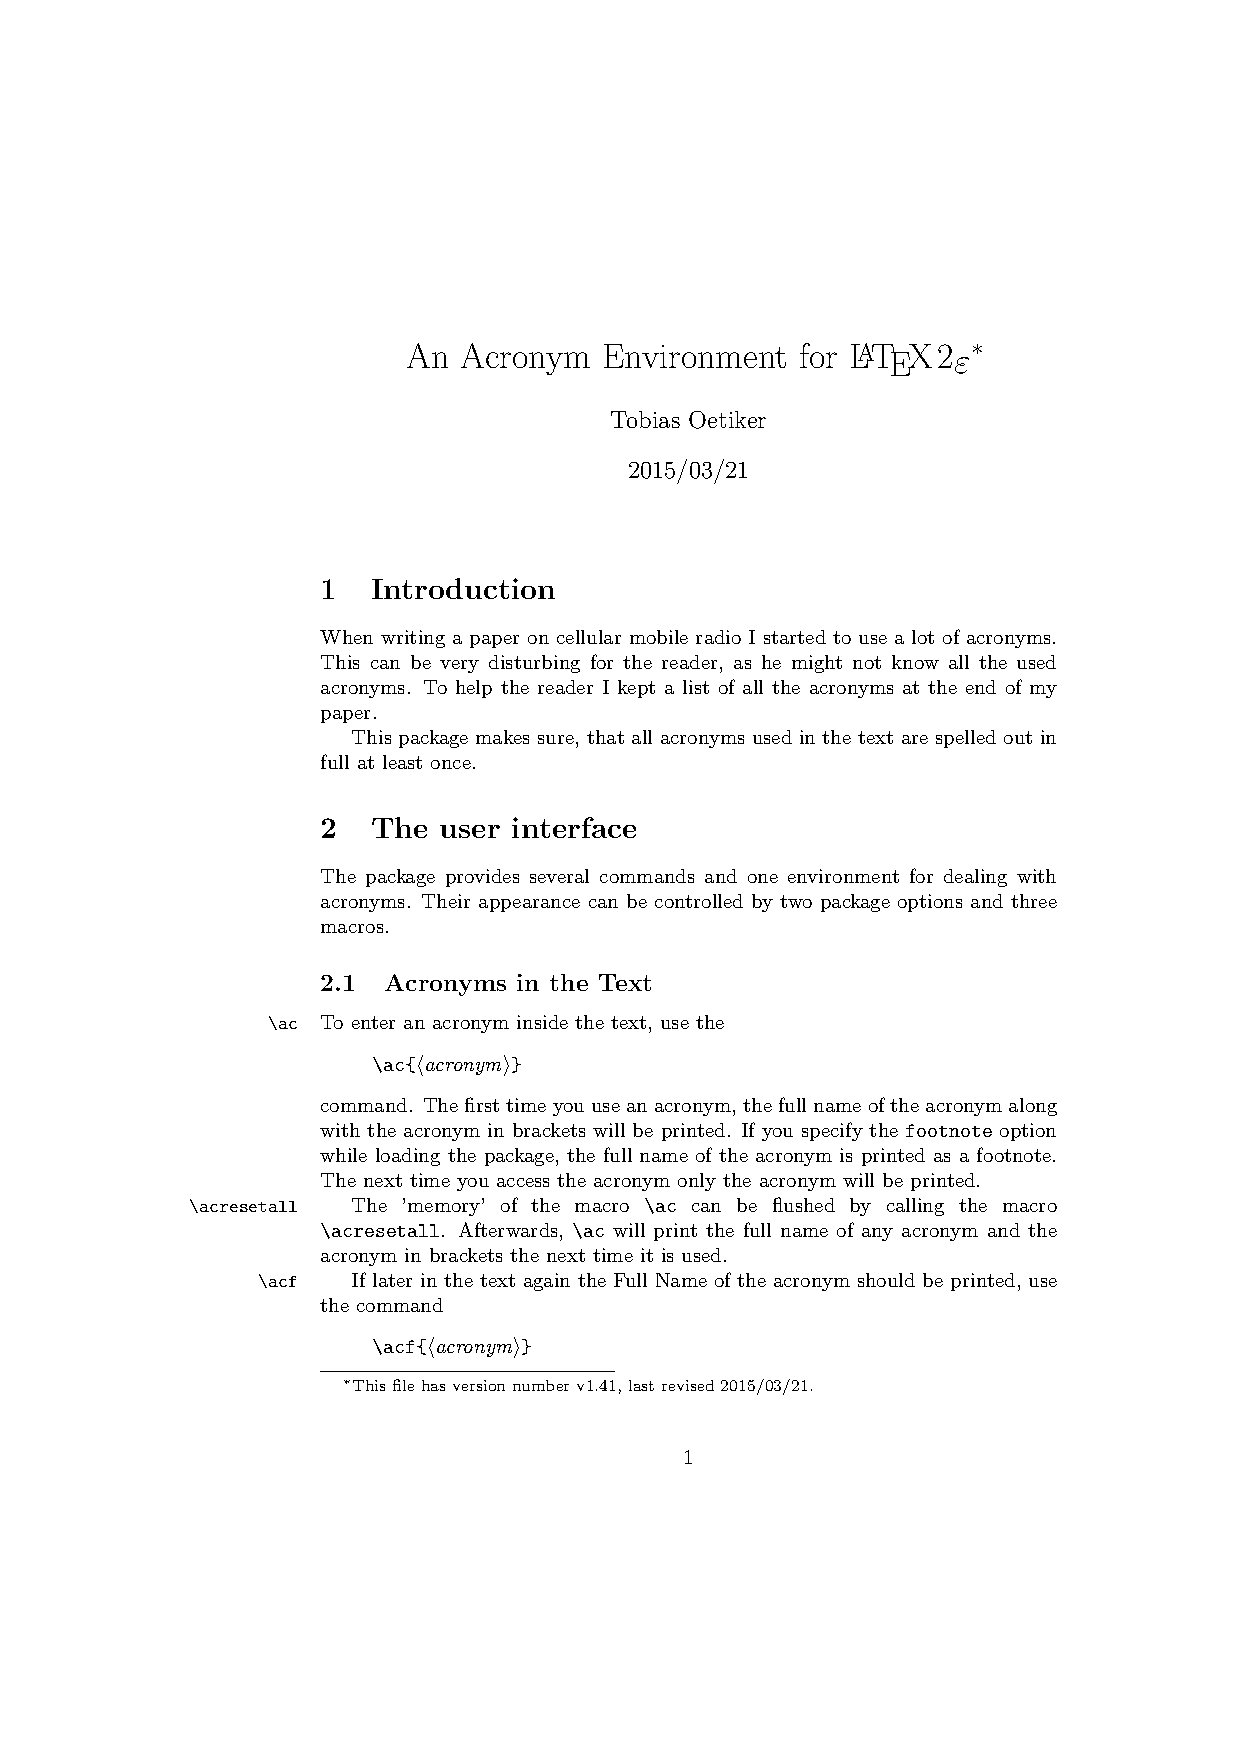
\includepdf[pages=1-3,frame=false,pagecommand={}]{anexos/acronym.pdf}



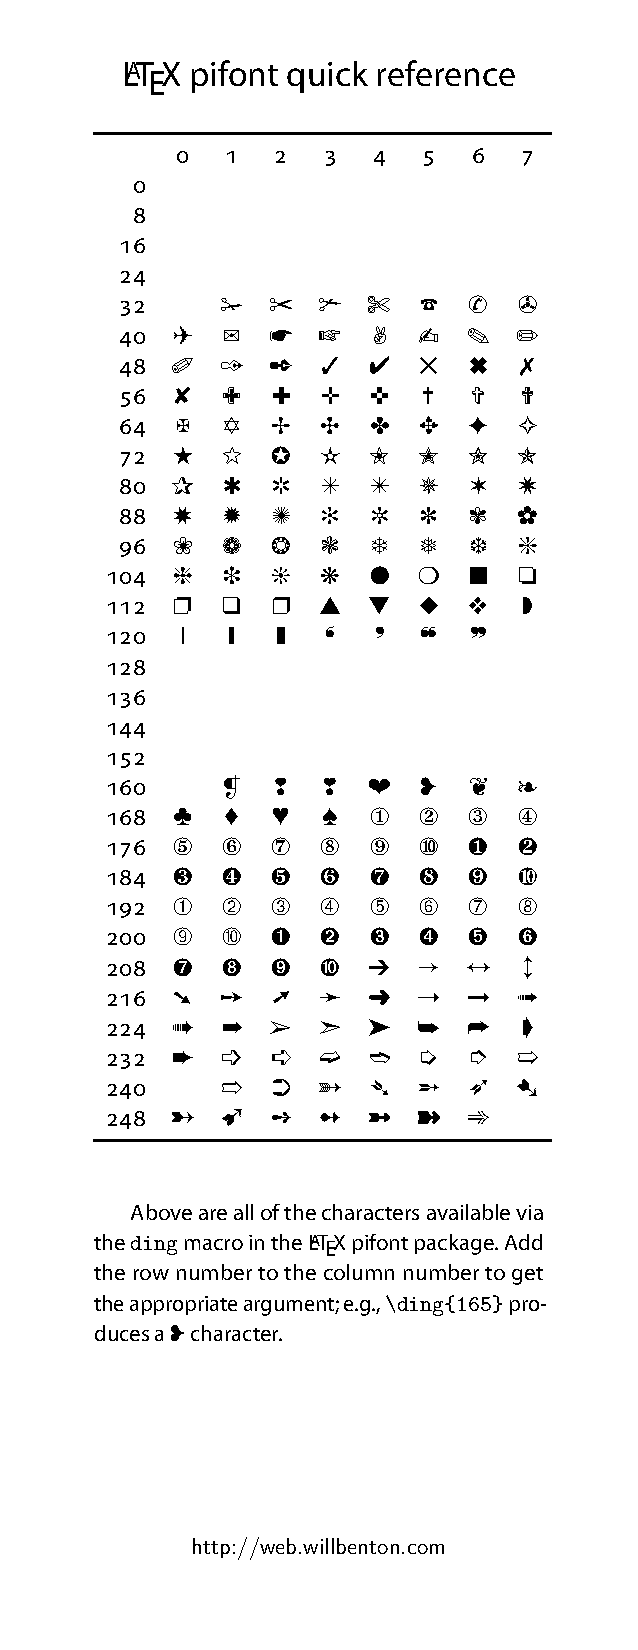
\includepdf[frame=true,scale=0.7,pagecommand=\chapter{Referência Rápida pifont}\label{pifont-quickref}]{anexos/pifont.pdf}
\end{comment}

\end{anexosenv}


\end{document}